\section{Introduction} 

\begin{definition}[\textit{Stochastic process}]
    A stochastic process (SP) is an infinite sequence of random variables, all defined on the same probabilistic space.
\end{definition}
A stochastic process can be represented as an infinite sequence:
\[\dots,v(1,s),v(2,s),v(3,s),\dots\]
Here, $s$ represents the realization of the random experiment, and it is the same for all elements of the sequence.

In general, each random variable in a sequence is indexed by $t$, representing the sequence index, and denoted by the realization of the random experiment, $s$.

When we set $s=\bar{s}$, we obtain a deterministic time signal. 
\begin{figure}[H]
    \centering
    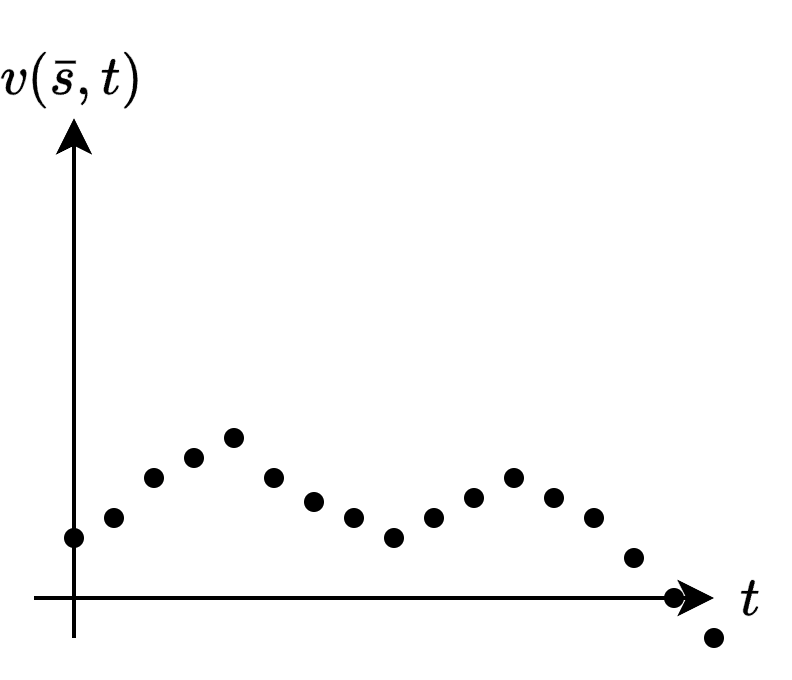
\includegraphics[width=0.35\linewidth]{images/outcome.png}
    \caption{Fixed realization}
\end{figure}
Alternatively, if we constrain the value of time to $t=\bar{t}$, we acquire a simple random variable. 
\begin{figure}[H]
    \centering
    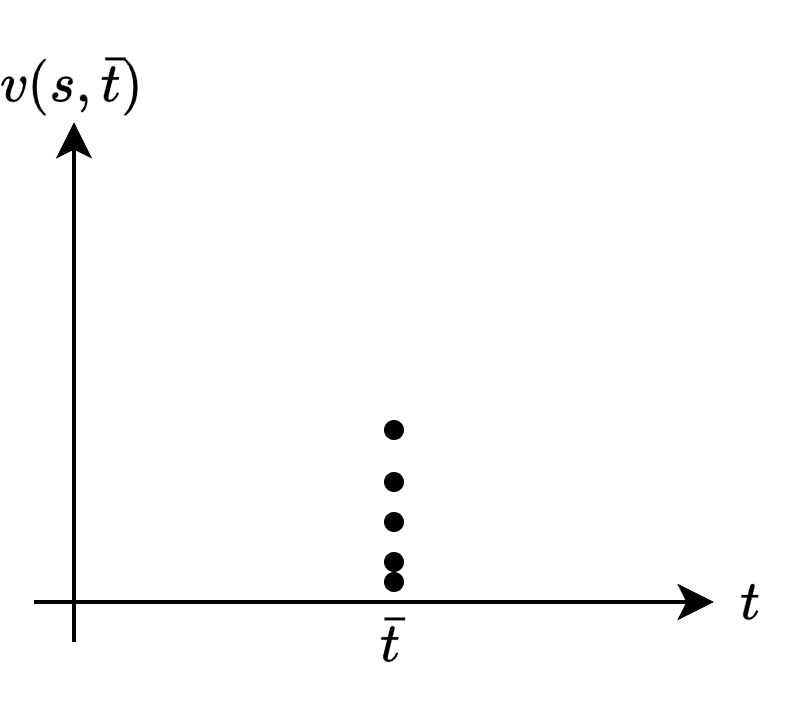
\includegraphics[width=0.35\linewidth]{images/time.png}
    \caption{Fixed time}
\end{figure}

\begin{definition}[\textit{Signal equivalence}]
    Two signals are considered equivalent from a stochastic perspective if they are realizations of the same stochastic process.
\end{definition}

\paragraph*{Wide-sense characterization}
A stochastic process is fully characterized by the probability distribution of $v(t,s)$.
 Wide-sense characterization is the description of a stochastic process solely through its mean and covariance functions.

\subsection{Mean value}
The mean value of a stochastic process $v(t,s)$ is defined as:
\[m(t)=\mathbb{E}\left[ v(t,s) \right]=\int_{\text{P}}v(t,s)pdf(s)\,ds\]
Graphically, the mean value can be computed by inspecting each time instant and determining the average point for each.

\subsection{Covariance function}
The covariance of a stochastic process $v(t,s)$ is defined as:
\[\gamma(t_1,t_2)=\mathbb{E}\left[ \left(v(t_1,s)-m(t_1)\right)\left(v(t_2,s)-m(t_2)\right) \right]\]
This function expresses the degree of correlation between two points at time instants $t_1$ and $t_2$.

\paragraph*{Variance}
When the two time instants coincide ($t_1=t_2=t$), we have:
\[\gamma(t_1,t_2)=\mathbb{E}\left[ \left(v(t_1,s)-m(t_1)\right)\left(v(t_2,s)-m(t_2)\right) \right]=\mathbb{E}\left[ {\left(v(t,s)-m(t)\right)}^2 \right] =\text{Var}\left[v(t,s)\right]=\gamma(\bar{s})\]
This function is referred to as the variance. 
It contains information about the variability of the stochastic process around its mean.